\capitulo{3}{Conceptos teóricos}

En mi experiencia como profesor de programación, diseño 3D y robótica para alumnos de primaria, lo primero que les enseñábamos era a definir la programación como el lenguaje de comunicación entre nosotros, los humanos, y los ordenadores o los robots. Todo esto pertenece a los conceptos más puramente teóricos sobre la computación y que es, en sí, la base de la informática. 

Pues bien, a <<grosso modo>> el concepto es el mismo ahora. Como cada uno, hombre y máquina, <<habla>> un idioma diferente se debe establecer un lenguaje que sea la vía de comunicación entre ambos. 

Para poder entender todo lo que se va a tratar a continuación, debo explicar primero el concepto de \textit{autómata} o \textit{máquina abstracta}. Un autómata es un modelo matemático o un dispositivo teórico que recibe una cadena de símbolos como entrada y que al procesarla, genera un cambio de estado produciendo una salida determinada. Esta salida pude reconocer palabras y determinar si la entrada pertenece a un determinado lenguaje o no. En el símil anterior digamos que es el corrector, que cuando escribe el humano algo determina si esta bien escrito o no porque no lo va a poder entender el ordenador. 

Entonces ya sabemos que para que haya comunicación entre un ordenador o robot y un humano, tiene que haber un lenguaje y un autómata. Pero también algo más: una gramática.

\section{¿ Qué es una gramática y para qué sirve?}

Una gramática formal es un mecanismo para la generación de cadenas de caracteres que son admitidas por un determinado lenguaje formal, y que utiliza un conjunto de reglas de formación. Por lo tanto, podemos entenderlo dentro del concepto de las ciencias de la computación y la lógica matemática. Las cadenas de caracteres resultantes son a su vez <<bien formadas>> cuando pertenecen al lenguaje formal con el que se trabaja.\cite{aho1986compilers}

¿ Y porque es tan importante? Siguiendo con el ejemplo del principio, la gramática es lo que va a determinar si lo que se introduce en el autómata es correcto o no. Un conjunto de reglas que nos indicará el porque al juntar una serie de caracteres de una forma se van a poder entender.

Por otro lado, la denominación de la gramática formal desde un punto de vista más concreto, de denomina como una cuádrupla compuesta por:

\begin{itemize}
	\item Un alfabeto de símbolos terminales o tókenes denominado con la letra griega $\Sigma$.
	\item $\mathcal{N}$ que es un alfabeto formado por símbolos no terminales
	\item Un alfabeto de producciones denominado $\mathcal{P}$.
	\item Y por último un símbolo llamado axioma o símbolo inicial el cual $\mathcal{S} \in \mathcal{N}$.
\end{itemize}

El alfabeto total que compone la gramática esta formado, según lo anterior, por $\Sigma\cup\mathcal{N}$ , es decir, por el conjunto de los símbolos terminales y no terminales.

Pongamos un ejemplo de una gramática simple y veamos de que esta formada. Se suele utilizar el sistema de notación  \[x \rightarrow y\] \[z \rightarrow w\] para indicar una o varias producciones, en vez de \[(x, y) \in \mathcal{P} \] \[(z, w) \in \mathcal{P} \] siendo $\mathcal{P}$ el conjunto de producciones.

Por otro lado si hay más de una producción que comience con el mismo elemento la notación sería de esta forma \[ x \rightarrow y | z | w\] en lugar de ser \[ x \rightarrow y, x \rightarrow z, x \rightarrow w\]


Producción: 

En aquellos proyectos que necesiten para su comprensión y desarrollo de unos conceptos teóricos de una determinada materia o de un determinado dominio de conocimiento, debe existir un apartado que sintetice dichos conceptos.

Algunos conceptos teóricos de \LaTeX \footnote{Créditos a los proyectos de Álvaro López Cantero: Configurador de Presupuestos y Roberto Izquierdo Amo: PLQuiz}.


queda por hacer todavia

\section{Cifrado de contraseñas y seguridad en Thoth Web}

El cifrado de la contraseña es una de las cuestiones más importantes para preservar la seguridad o intimidad del usuario. El porqué es muy simple. Los usuarios normalmente utilizamos las mismas contraseñas o parecidas para cualquier cuenta de una página o red social. Por lo tanto si hay alguien con acceso a la base de datos, podrá ver la contraseña utilizada por un determinado usuario poniendo en peligro esa intimidad no solo en este programa, sino, como ya se ha comentado antes, la de otras cuentas.

Para evitar esto, el método más simple es el cifrar las contraseñas en la base de datos para que en el caso en el que alguien acceda a ella, en el campo <<contraseña>> no vea la contraseña real, sino el resultado del cifrado de esta. El método de cifrado que se emplea en Thoth Web el del algoritmo <<hash>> que como veremos más adelante tiene unas características determinadas. 

\subsection{Funcionamiento del algoritmo hash}

Se trata de un algoritmo matemático con el que se transforma cualquier cantidad de datos en una serie de datos fija que funciona como una huella dactilar. Esto quiere decir que sea cual sea la cantidad de caracteres de entrada, la salida siempre será fija. Cumple además con dos premisas muy importantes para la seguridad: 

\begin{itemize}
\item No es reversible, no se puede descifrar por medio de funciones matemáticas y obtener el resultado antes de ser encriptado, sea cual sea la función utilizada (SHA-1, SHA-2 o MD 5 entre otras, como veremos a continuación).
\item Cuenta con la propiedad de que si la entrada cambia, aunque sea sólo en un bit, el hash resultante será completamente, como se puede ver en la siguiente ilustración \ref{fig:3.1}. En la imagen se puede apreciar que aunque la entrada tenga un mayor numero de caracteres, la salida siempre sera de 40 caracteres.

\end{itemize} 

\begin{figure}[h]
\centering
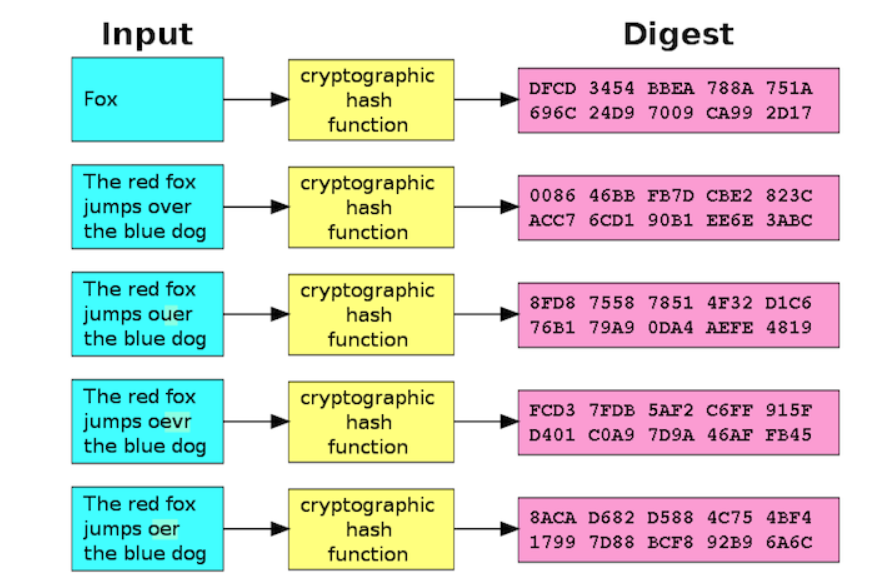
\includegraphics[width=0.99\textwidth]{funcion-hash}
\caption{Aplicación de la función hash a diferentes datos introducidos.}
\label{fig:3.1}
\end{figure}

Ahora bien, las acciones llevadas a cabo para preservar esa seguridad serian las siguientes: un usuario crea una cuenta en la aplicación, la contraseña se encripta y se almacena en la base de datos. Cuando el usuario trata de iniciar sesión y escribe la contraseña, esta se encripta y se compara el resultado con aquel que se ha guardado en la base de datos, si son iguales el usuario tendrá acceso sino, se le requerirá que lo vuelva a intentar.

El problema principal de esto es que con los avances en temas de seguridad siempre hay asociados otros que tratan de <<romper>> esa seguridad y en este caso no iba a ser menos. Creo que es importante reconocer los peligros que hay asociados a aplicar este método, pero no deseo extenderme demasiado en este aspecto así que los mencionare brevemente.


\begin{itemize}
\item Ataques de fuerza bruta. Consisten en utilizar diccionarios de palabras con contraseñas habituales e introducirlas hasta que alguna coincida. Se trata del ataque menos eficiente, pero el más difícil de evitar.
\item Tablas de búsqueda. Este tipo de ataque si que supondría un grave problema para la seguridad en el cifrado con algoritmo hash. Recordemos que las funciones hash solo se pueden encriptar, no descifrar. Lo que hace este ataque es lo siguiente, cuenta con una tabla de contraseñas típicas y su cifrado hash y las compara con los hash introducidos. Para entender mejor este concepto hay incluso herramientas online que pueden hacer este trabajo \ref{fig:3.2}. También las hay que funcionan al revés. Introduces la contraseña que crees que puede usar alguien, la encripta, la compara con todas las de la base de datos y te dice si alguien la utiliza o no.
\end{itemize}

\begin{figure}[h]
\centering
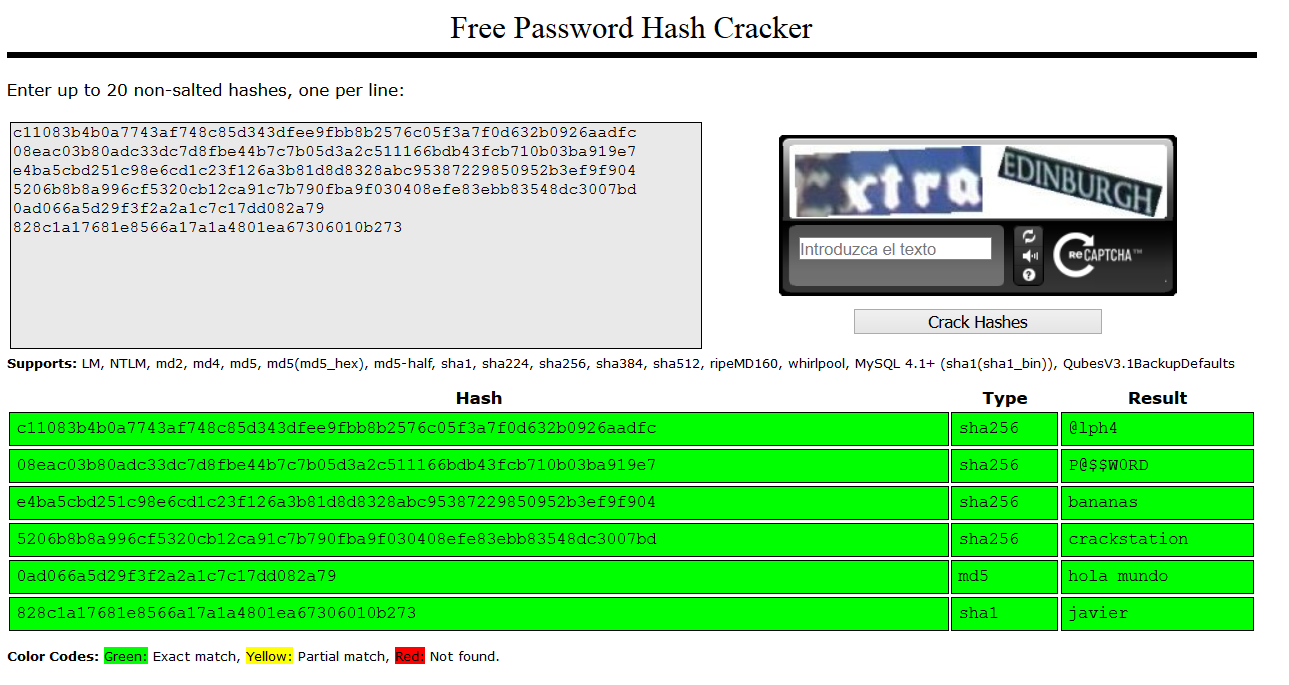
\includegraphics[width=0.99\textwidth]{hash-cracker}
\caption{Ejemplo de ataque con tablas de búsqueda.}
\label{fig:3.2}
\end{figure}

Además de estos, hay más métodos, casi todos basados en las tablas de búsqueda. Según estos ataques queda comprobado que la seguridad de este algoritmo depende en gran mediada de la contraseña que utilice el usuario. Cuanto más aleatoria y con más mezcla de caracteres mejor, ya que formará palabras que no se encuentran en los diccionarios o tablas y solo se podrá descubrir por medio de la fuerza bruta. Entonces ¿ cómo hacer que las contraseñas sean más resistentes y solucionar este problema?

Se conoce como el cifrado hash con sal o semilla. Consiste en añadir un conjunto de caracteres aleatorios, agregarlos a la contraseña y una vez hecho esto, cifrarlo con la función hash. De esta manera se consigue que la contraseña sea mucho más aleatoria que la que inicialmente ha introducido el usuario. Así podemos ver como quedaría un intento de <<tablas de búsqueda>> con este tipo de cifrado usa para contraseñas muy simples \ref{fig:3.3}. 

\begin{figure}[h]
\centering
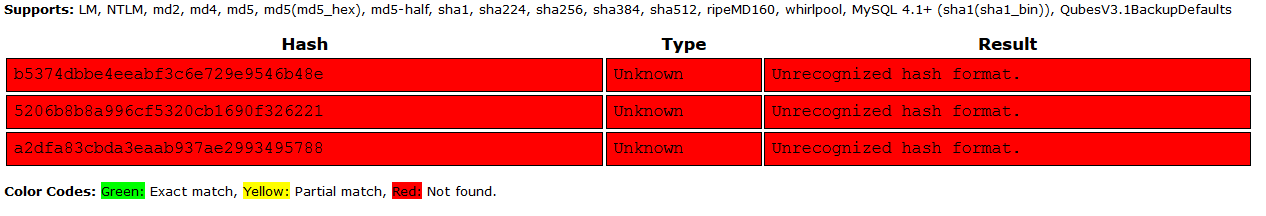
\includegraphics[width=0.99\textwidth]{hash_salt-cracker}
\caption{Resultado de aplicar tablas de búsqueda al cifrado hash con semilla.}
\label{fig:3.3}
\end{figure}

La primera de ellas corresponde con la clave <<123>> la segunda con la palabra <<contraseña>> y la tercera con la fecha <<16-6-17>>. Todas son fáciles, pero al añadirle una clave y cifrarlo todo, se vuelve mucho mas complejo. Se podría pensar que, como la clave que se le añade también se guarda en la base de datos sigue sin ser seguro. Partiendo del hecho de que no hay prácticamente nada seguro al cien por cien, lo que se consigue con esto es dificultar mucho el cálculo y con este método se consigue de una forma muy simple.



\subsection{Subsecciones}

Además de secciones tenemos subsecciones.

\subsubsection{Subsubsecciones}

Y subsecciones. 


\section{Referencias}

Las referencias se incluyen en el texto usando cite \cite{wiki:latex}. Para citar webs, artículos o libros \cite{koza92}.


\section{Imágenes}

Se pueden incluir imágenes con los comandos standard de \LaTeX, pero esta plantilla dispone de comandos propios como por ejemplo el siguiente:

\imagen{escudoInfor}{Autómata para una expresión vacía}



\section{Listas de items}

Existen tres posibilidades:

\begin{itemize}
	\item primer item.
	\item segundo item.
\end{itemize}

\begin{enumerate}
	\item primer item.
	\item segundo item.
\end{enumerate}

\begin{description}
	\item[Primer item] más información sobre el primer item.
	\item[Segundo item] más información sobre el segundo item.
\end{description}
	
\begin{itemize}
\item 
\end{itemize}

\section{Tablas}

Igualmente se pueden usar los comandos específicos de \LaTeX o bien usar alguno de los comandos de la plantilla.

\tablaSmall{Herramientas y tecnologías utilizadas en cada parte del proyecto}{l c c c c}{herramientasportipodeuso}
{ \multicolumn{1}{l}{Herramientas} & App AngularJS & API REST & BD & Memoria \\}{ 
HTML5 & X & & &\\
CSS3 & X & & &\\
BOOTSTRAP & X & & &\\
JavaScript & X & & &\\
AngularJS & X & & &\\
Bower & X & & &\\
PHP & & X & &\\
Karma + Jasmine & X & & &\\
Slim framework & & X & &\\
Idiorm & & X & &\\
Composer & & X & &\\
JSON & X & X & &\\
PhpStorm & X & X & &\\
MySQL & & & X &\\
PhpMyAdmin & & & X &\\
Git + BitBucket & X & X & X & X\\
Mik\TeX{} & & & & X\\
\TeX{}Maker & & & & X\\
Astah & & & & X\\
Balsamiq Mockups & X & & &\\
VersionOne & X & X & X & X\\
} 
